\section{The two-photon vertex of NRQED}
%TODO cleanup notation
In the NRQED Lagrangian, in addition to the terms involving the fermions interaction with a single photon, there are terms which represent the interaction of a fermion with two photons.  At the order needed, all such terms are fixed by gauge invariance.  There are terms, such as those involving $\v{E}^2$, that would are by themselves gauge invariant, but these occur at too high an order.  (The order of such a term would be $E^2 / m^3 \sim mv^6$.)

So though the coefficients of concern are all fixed by considering just the one-photon interactions, they could also be fixed from considering two-photon interactions.  Since it \emph{is} possible, it makes sense to do so, as a check of consistency.  In this section, the coefficients of two-photon terms in the NRQED Lagrangian will be fixed from QED calculations.

As before, this will involve calculating some physical process in both QED and NRQED, and comparing the result.  The simplest two photon process to consider is Compton scattering.  By calculating Compton scattering in each theory, the coefficients desired will be obtained.

This is not quite as straightforward as in the case of the one-photon scattering, for the following reason: while the one-photon scattering is a local interaction in both QED and NRQED, Compton scattering will involve some mix of local and non-local diagrams.  In QED, there are of course no local interactions between a fermion and two photons.  The situation is most readily stated diagrammatically.

In QED, the leading order diagrams contributing to Compton scattering are:

\vspace{1em}
 \mbox{
\begin{minipage}{1.6in}
   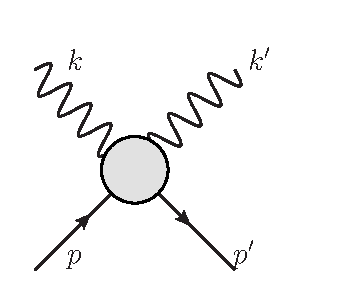
\includegraphics[scale=0.8]{eps/2photon-blob} 
\end{minipage}
$	=	\hspace{2em} 	 $
\begin{minipage}{1.6in}
   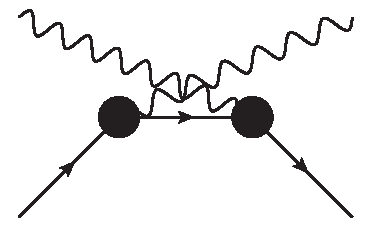
\includegraphics[scale=0.8]{eps/Tree-crossed}
\end{minipage}
$\hspace{2em}   +  \hspace{2em} $
\begin{minipage}{1.6in}
   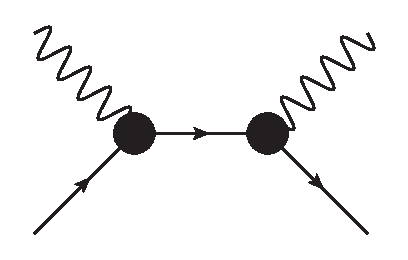
\includegraphics[scale=0.8]{eps/Tree-uncrossed} 
\end{minipage}
} 
\vspace{1em}



While in NRQED, the following diagrams contribute to the scattering:

\vspace{1em}
 \mbox{
\begin{minipage}{1.6in}
   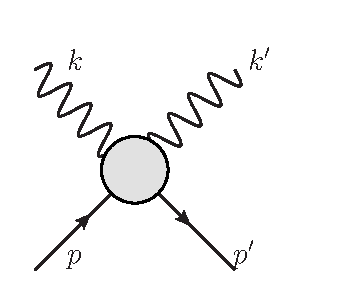
\includegraphics[scale=0.8]{eps/2photon-blob} 
\end{minipage}
$	=	\hspace{2em} 	 $
\begin{minipage}{1.6in}
   %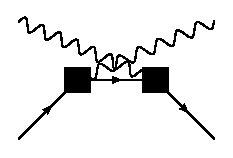
\includegraphics[scale=0.8]{eps/Tree-crossed-square}
\end{minipage}
$\hspace{2em}   +  \hspace{2em} $
\begin{minipage}{1.6in}
   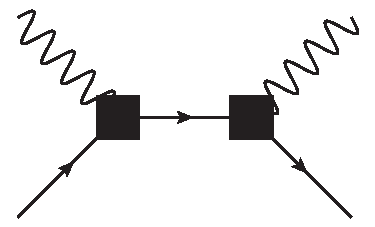
\includegraphics[scale=0.8]{eps/Tree-uncrossed-square} 
\end{minipage}
} 
\vspace{1em}



In each set of diagrams, the vertices represent the \emph{total} electron vertex.  For QED this is determined, as before, by the form factors, and for NRQED it is determined by the calculations of the previous section.

Since the two amplitudes must be equal, in principle the process is this: First calculate the scattering amplitude in QED.  Then, calculate the contribution to the scattering amplitude coming from the tree diagrams I and II above.  Whatever discrepancy remains must be the value of the local two-photon vertex III.   

The process of subtracting the one set of diagrams from the other could be slightly complicated, but luckily it turns out there is a simpler path.  By considering the physical origin of the local terms in NRQED, it will be possible to split the QED diagrams into local and non-local parts, where the latter can be shown to be equal to the non-local diagrams in NRQED.  Then, comparing the two scattering processes becomes much easier.

\subsubsection{Z diagrams}
The high energy theory (QED) doesn't contain any two-photon vertices, while the low energy theory (NRQED) does.  This is a general feature of effective field theories, that new types of local interactions arise.  The high energy theory can have intermediate states that are highly virtual, while the low energy theory doesn't.  Instead, as according to the uncertainty principle, intermediate states with extremely high energy can be considered to occur almost instantaneously, giving rise in the effective theory to local interactions.

How does the local two-photon interaction arise in NRQED?  Of course there are an infinite number of contributions, but we'll consider just the leading order contributions.  These will come from the tree level two photon diagrams as shown above.  Compare the tree-level diagrams in the two theories: in addition to the vertices being different, so are the propagators.  The propagator in QED represents some admixture of the electron and positron field, while in NRQED it is only the electron.
%%%%%%%%
In both QED and NRQED, a process is calculated as the sum of a series of diagrams, representing an expansion in perturbation theory.  However, there is a difference btween the two in the nature of perturbation theory employed.

In QED, at each vertex both energy and momentum is conserved.  But intermediate particles may be off mass-shell; that is, it is no longer the case that for a particle of four-momentum $p$ and mass $m$ that $p^2 = m^2$.

In NRQED, the old Rayleigh-Schrodinger perturbation theory is used.   All intermediate particles are on mass-shell.  But at the vertices (when represented diagrammatically), although momenta is conserved, energy is not.  


Remember that in old perturbation theory, corrections have the rough form
\beq
	\Delta =  \Sigma_\text{int} \frac{  \matrixel{\text{out} }{V}{\text{int}} \matrixel{\text{int} }{V}{\text{in}} }{E_\text{in} - E_\text{int}}
	%\Delta = \frac{  \matrixel{A}{B}{C} }{E - E}
\eeq
where the sum is over intermediate states, which can have differing energy from the initial state.

The trick, then is to take the relativistic tree-level diagrams of QED and rewrite them in the language of  Rayleigh-Schrodinger before trying to compare them to NRQED.  In NRQED, only intermediate states involving electrons can be considered, but in QED intermediate states identified with positrons will appear as well.  It is \emph{these} processes, involving a large violation of energy conservation, that will appear as contact terms in NRQED.  

There are two diagrams in QED, and both can be dealt with in the same general way.  Consider the uncrossed diagram:

%TODO fix diagrams


\vspace{1em}
 \mbox{
\begin{minipage}{1.6in}
   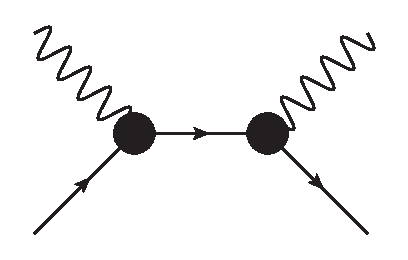
\includegraphics[scale=0.8]{eps/Tree-uncrossed} 
\end{minipage}
$	 \hspace{2em} =		 $
\begin{minipage}{1.6in}
   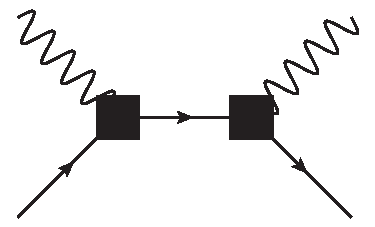
\includegraphics[scale=0.8]{eps/Tree-uncrossed-square}
\end{minipage}
$\hspace{2em}   +  \hspace{2em} $
\begin{minipage}{1.6in}
   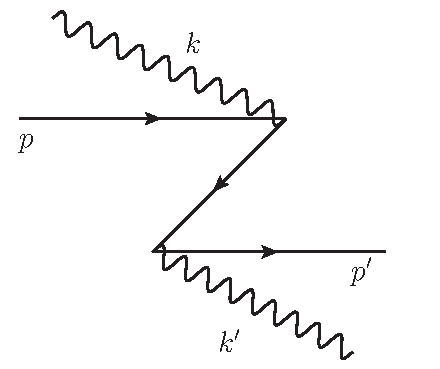
\includegraphics[scale=0.8]{eps/Zdiag} 
\end{minipage}
} 
\vspace{1em}



There are two tree level processes that can be considered in the old time-ordered perturbation theory.  The first corresponds to an incoming electron, which first absorbs a photon and then emits one.  The second, more complicated process, involves the creation of intermediate positron.  While a free electron travels along, an incoming photon decays into an electron and positron.  Then, the positron annihilates the incoming electron and emits the outgoing photon.  Because of the shape of this diagram, it is called a ``Z diagram.''

In the Z-diagrams, the electrons and the photons are external, so the sum over the intermediate states is specifically the intermediate states of the positrons.  Likewise, the other diagrams are written as a sum over intermediate electron states.  But because of the rules of Rayleigh-Schrodinger perturbation theory, all these states are on mass shell.  And since the momenta here is fixed, the sum over intermediate states is a sum over spin states.

So the original QED diagram should somehow split into two terms, one involving a sum over electron states and the other a sum over anti-particles.  

%TODO insert diagram
Call the intermediate momentum $\v{q}$.  The initial energy will be $q_0$, the intermediate energy will be that of the on mass shell particle, $E_q = \sqrt{\v{q}^2 + m^2 }$.


\vspace{1em}
 \mbox{
\begin{minipage}{1in}
   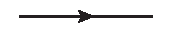
\includegraphics[scale=0.8]{eps/prop} 
\end{minipage}
$	=$ \hspace{1em} $	i\frac{ \cancel{q} -m}{q^2 - m^2}  
		= i\frac{1}{\sqrt{\v{q}^2 + m^2} } \left(
			\frac{ \Sigma \bar{u}(\v{q}) u(\v{q}) }  {q_0 - \sqrt{\v{q}^2 + m^2} }
			+ \frac{ \Sigma \bar{v}(-\v{q}) v(-\v{q}) }  {q_0 + \sqrt{\v{q}^2 + m^2} }
		\right )	 $
} 
\vspace{1em}




This identity can be technically reproduced as follows.  First write the denominator of the propagator as
\beq
	i\frac{ \cancel{q} -m}{q^2 - m^2}   = i \frac{ \cancel{q} -m}{q_0^2 -(\v{q}^2 + m^2)}
\eeq
This could be factored into 
\beq
	q_0^2 -(\v{q}^2 + m^2) = (q_0 + \sqrt{\v{q}^2 + m^2})  (q_0 - \sqrt{\v{q}^2 + m^2})
\eeq
So it implies poles at $q_0 = \pm  \sqrt{\v{q}^2 + m^2}$.  There is one unique way of factoring the original propagator into the two poles:
\beq
	\frac{1}{2\sqrt{\v{q}^2 + m^2}}
		\left(
			\frac{ \gamma^0 \sqrt{\v{q}^2 + m^2} - \v{\gamma} \cdot \v{q} + m}{q_0 - \sqrt{\v{q}^2 + m^2}}
			- \frac{ \gamma^0 \sqrt{\v{q}^2 + m^2} + \v{\gamma} \cdot \v{q} - m}{q_0 + \sqrt{\v{q}^2 + m^2}}
		\right)
\eeq
The two numerators can be exactly equated to sums over polarisation states of electron and positron spinors:
\beqa
	\Sigma u(\v{p}) \bar{u}(\v{p}) &=& \gamma \cdot p + m	\\
	\Sigma v(\v{p}) \bar{v}(\v{p}) &=& \gamma \cdot p - m	\\
\eeqa
These relations hold for particles which are on mass-shell.  That is exactly the case here.  But then, there is an assumption that the quantity $p_0$ above is the on mass-shell energy, $\sqrt{\v{p}^2 + m^2}$.

So, noting that particles with momentum $\pm \v{q}$ have the same energy $\sqrt{\v{q}^2 + m^2}$ and that $q_0$ is the off-mass shell energy from the relativistic diagram, the propagator can be rewritten:
\beq
	\frac{1}{2\sqrt{\v{q}^2 + m^2}}
		\left(
			\frac{\Sigma u(\v{q}) \bar{u}(\v{q}) }{q_0 - \sqrt{\v{q}^2 + m^2}}
			- \frac{  \Sigma v(-\v{q}) \bar{v}(-\v{q})}{q_0 + \sqrt{\v{q}^2 + m^2}}
		\right)
\eeq
The numerators have now been put into exactly the forms expected for the regular- and Z-diagrams of old perturbation theory. 


As mentioned above this can be understood in the context of old perturbation theory as sum over intermediate states in the numerator,  with the expected form of the denominator being $E_\text{in} - E_\text{int}$.  It can be shown that the denominators have exactly this form. 

Now consider the first, regular diagram.  The initial energy is $q_0$, since in relativistic theory the total energy at the vertex is conserved.  The intermediate energy is the on-mass shell energy of the electron: $\sqrt{\v{q}^2+ m^2}$.  Thus the denominator of $q_0 - \sqrt{\v{q}^2+ m^2}$ is that expected.

Now consider the Z-diagram.  The initial energy is still $q_0$.  The intermediate energy is more complicated: there are two photons, two electrons, and a positron present.  The total combined energy is:
\beq
	E_\text{int} = p_0 + p'_0 + k_0 + k'_0 + \sqrt{\v{q}^2 + m^2} = 2q_0 +  \sqrt{\v{q}^2 + m^2}
\eeq
Then the difference $E_\text{in} - E_\text{int} = -q_0 - \sqrt{\v{q}^2 + m^2}$, as expected.

So rewriting the propagator into these two separate terms can be understood as how the fully relativistic process appears in old perturbation theory.  In a relativistic theory, intermediate states involving positrons must be accounted for.  For higher order QED diagrams more complicated processes will appear, but at the tree level only those discussed above are involved.  No approximations are involved --- the identity for the propagator is exact.  The form is more convenient for discussing nonrelativistic energies, but is still equivalent to the relativistic diagrams.

%Four equations for each of the diagrams





\subsubsection{Relation between NRQED and old perturbation theory}
Now it is necessary to show how the diagrams in old perturbation theory relate to those of NRQED.  

The normal diagrams can be easily interpreted as the product of vertices and the relativistic Rayleigh-Schrodinger propagator:
%Equation with diagram on left, prodcut of verices on right

\vspace{1em}
 \mbox{
\begin{minipage}{1.6in}
   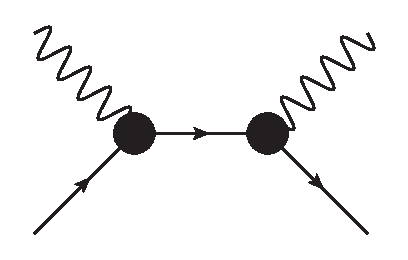
\includegraphics[scale=0.8]{eps/Tree-uncrossed} 
\end{minipage}
$	=	\hspace{2em} 	\Bigg( $
\begin{minipage}{1.0in}
   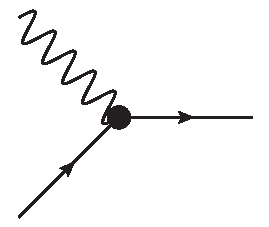
\includegraphics[scale=0.6]{eps/vertex-in}
\end{minipage}
$\Bigg ) \times \Bigg ($
\begin{minipage}{0.8in}
   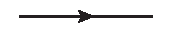
\includegraphics[scale=0.9]{eps/prop} 
\end{minipage}
$\Bigg ) \times \Bigg ($\begin{minipage}{1.0in}
   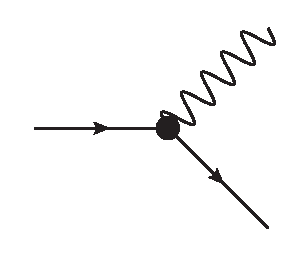
\includegraphics[scale=0.6]{eps/vertex-out} 
\end{minipage}
$\Bigg )$
} 
\vspace{1em}
 



Where
%Define each piece
%Vertex in, prop, vertex out
Recall that the total NRQED one-photon vertex was derived by comparing to the QED vertex, so necessarily
\beq
	\bar{u} \Gamma^0 u = \phi^\dagger V^0 \phi , \;  \bar{u} \Gamma^i u = \phi^\dagger V^i \phi
\eeq 
The propagator $1/(q_0 - \sqrt{m^2 + \v{q}^2})$ is equal to the total propagator in NRQED (including relativistic corrections).  So it really is the case that the two sets of diagrams are equivalent.  Whether the vertices are written in terms of NRQED or QED, the ultimate expression will be the same.

It then follows that the contributions to the local contact term in NRQED come (at tree level) exactly from the Z-diagrams.  To calculate the contact terms to the order (in the nonrelativistic expansion) needed, the Z-diagrams need to be approximated just as the one-photon vertex diagrams were in the previous section.  Then the NRQED coefficients can be obtained by comparing the two calculations.  

At nonrelativistic energies, it would be expected that the sum over intermediate states now does not resemble a propagator.  Because only terms involving up to one power of momentum need be kept, the square root term becomes simply $m$.  $q_0$, the total incoming energy, will involve both the electron and photon energy.  Depending on whether the crossed or uncrossed diagram is considered, it will be either $q_0 = p_0 + k_0$ or $q_0 = p_0 - k'_0$.  In either case, it will be $m$ at the leading order, with a first order correction due to the photon energy. 
\beq
	\frac{ \Sigma \bar{v}(-\v{q}) v(-\v{q}) }  {q_0 + \sqrt{\v{q}^2 + m^2} } 
		\approx \frac{ \Sigma \bar{v}(-\v{q}) v(-\v{q}) }  {2m + (q_0-m) }
\eeq
Since $q_0-m << m$, this can then be written as 
\beq
		\approx  \left( 1 - \frac{q_0-m}{2m} \right ) \frac{ \Sigma \bar{v}(-\v{q}) v(-\v{q}) }  {2m}
\eeq
In this approximation, the two Z diagrams become


\vspace{1em}
 \mbox{
\begin{minipage}{1.6in}
   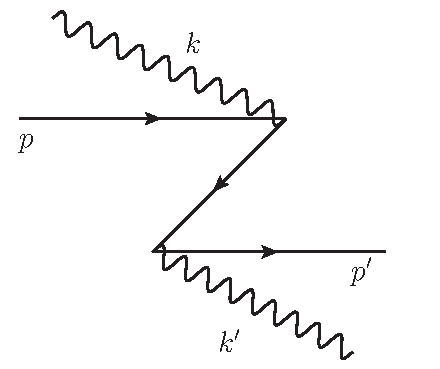
\includegraphics[scale=0.6]{eps/Zdiag} 
\end{minipage}
= \hspace{1em}
$	
\Sigma_{\text{spin}}
\left( 1 - \frac{k_0}{2m} \right ) \frac{1}{2m} 
	\bar{u}(\v{p'}) \gamma^\mu \epsilon^*_\mu(k') v_s(-\v{p} - \v{k}) \bar{v}_s(-\v{p} - \v{k}) \Gamma^\nu \epsilon_\nu(k) u(\v{p})
$
} 
\vspace{1em}


\vspace{1em}
 \mbox{
\begin{minipage}{1.6in}
   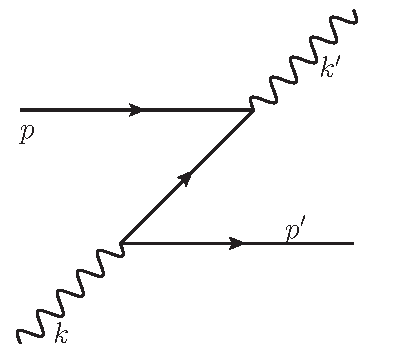
\includegraphics[scale=0.6]{eps/Zdiag2} 
\end{minipage}
= \hspace{1em}
$	
\Sigma_{\text{spin}}
\left( 1 + \frac{k'_0}{2m} \right ) \frac{1}{2m} 
	\bar{u}(\v{p'}) \gamma^\mu \epsilon_\mu(k) v(\v{k'} - \v{p})_s \bar{v}_s(\v{k'} - \v{p}) \Gamma^\nu \epsilon^*_\nu(k') u(\v{p})
$
} 
\vspace{1em}

While the sums over intermediate states could also be expanded, it'll be easiest to calculate these in the above form.  The vertices will be the sum of particle-antiparticle bilinears, which can be calculated separately.



\subsection{Nonrelativistic expressions for Z diagrams}


Looking at the equations for the Z diagrams, they are both the product of two types of terms to calculate:

\beq \label{eq:Sh:uvGamma}
	\bar{u}(\v{p'}) \Gamma^\mu(q) v(\gv{\ell}) \;  \text{and} \; \bar{u}(\gv{\ell}) \Gamma^\mu(q) v(\v{p})
\eeq
Here $\ell$ is the intermediate momentum of the positron, and $q$ is the momentum of the photon going into the vertex (either $k$ or $-k'$).  The form of $\Gamma$ is
\beq
	\Gamma^\mu(q) = F_1 \gamma^\mu + F_2 \frac{q_\nu \sigma^{\mu\nu}}{2m}
\eeq
To compare the Z diagrams to the contact terms of NRQED, first express the bilinears in the vertices of \eqref{eq:Sh:uvGamma} in terms of the nonrelativistic quantities.  This can be done for each of the two terms in $\Gamma^\mu$ separately.  The bispinors $u$ will be replaced by the spinor $\phi$, as before.  Now, the bispinor $v$ will be replaced by a spinor for a positron, which shall be called $\chi$.  In doing the expansion only terms up to $\mathcal{O}(1/m)$ need be kept.


To calculate the vector like bilinears, treat the spatial and time-like components separately.  First $\mu=0$:
\beqa
	\ubar(p') \gamma^0 v(\ell)
		&=&	\udaggervec{\v{p'}} \vvec{\v{q}}	\\
		&=&	\phi^\dagger \left( \frac{ \sigdot{\ell} + \sigdot{p'} }{2m} \right ) \chi	\\
	\vbar{\ell} \gamma^0 u(p)
		&=&	\vdaggervec{\ell} \uvec{p}	\\
		&=&	\chi^\dagger \left( \frac{ \sigdot{\ell} + \sigdot{p} }{2m} \right ) \phi	
\eeqa
Then $\mu=i$:
\beqa
	\ubar(p') \gamma^i v(\ell)
		&=&	\udaggervec{p'} \begin{pmatrix} 0 & \sigma_i \\ \sigma_i & 0 \end{pmatrix} \vvec{\ell}	\\
		&=&	\phi^\dagger \sigma_i \chi \\
	\vbar(\ell) \gamma^i u(p)
		&=&	\vdaggervec{\ell} \begin{pmatrix} 0 & \sigma_i \\ \sigma_i & 0 \end{pmatrix} \uvec{p}	\\
		&=&	\chi^\dagger \sigma_i \phi 
\eeqa

In the tensor terms a factor of momentum $q_\nu$ appears.  The spatial part, $q_j$ is ``naturally raised" so $q_j = -(\v{q})_j$.  As before the two types of indices should be treated separately.  For $\mu=0$:

\beqa
	\frac{i q_\nu}{2m} \ubar(p') \sigma^{0 \nu} v(\ell) 
		&=& \frac{i q_j}{2m} \ubar(p') \sigma^{0j} v(\ell) \\
		&=& -\frac{q_j}{2m} \udaggervec{p'} \Mblock{0}{\sigma^i}{-\sigma^i}{0} \vvec{\ell}	\\
		&=& \phi^\dagger \frac{ \sigdot{q}}{2m} \chi	\\
	\frac{i q_\nu}{2m} \vbar(\ell) \sigma^{0 \nu} u(p) 
		&=& \frac{i q_j}{2m} \vbar(\ell) \sigma^{0j} u(p) \\
		&=& -\frac{q_j}{2m} \vbar{\ell} \Mblock{0}{\sigma^i}{-\sigma^i}{0} \uvec{p}	\\
		&=& -\chi^\dagger \frac{ \sigdot{q}}{2m} \phi	\\
\eeqa
Then for $\mu=i$
\beq
	\frac{i q_\nu}{2m} \ubar(p') \sigma^{i \nu} v(\ell)
	 	= \frac{i q_0}{2m} \ubar(p') \sigma^{i 0} v(\ell) + \frac{i q_j}{2m} \ubar(p') \sigma^{i j} v(\ell)	
\eeq
\beq
	 = - \frac{i q_0}{2m}  \udaggervec{p'} \Mblock{0}{\sigma^i}{-\sigma^i}{0} \vvec{\ell} 	
	 	+ \frac{i q_j}{2m}  \epsilon_{ijk}  \udaggervec{p'} \Mblock{\sigma^k}{0}{0}{\sigma^k} \vvec{\ell} \nonumber
\eeq
The second term will be of order $\mathcal{O}(1/m^2)$ and so can be neglected.  So 
\beq
	\frac{i q_\nu}{2m} \ubar(p') \sigma^{i \nu} v(\ell) 
		= \phi^\dagger \frac{q_0 \sigma_i}{2m} \chi
\eeq
The complementary term is 
\beq
	\frac{i q_\nu}{2m} \vbar(\ell) \sigma^{i \nu} u(p)
	 	= \frac{i q_0}{2m} \vbar(\ell) \sigma^{i 0} v(\ell) + \frac{i q_j}{2m} \ubar(p') \sigma^{i j} u(p)	
\eeq
Again,  the second term with $\sigma^{ij}$ has the same general structure and will be of order $1/m^2$.  So 
\beqa
		\frac{i q_\nu}{2m} \vbar(\ell) \sigma^{i \nu} u(p)
	 &=&	\frac{i q_0}{2m} \vdaggervec{\ell} \Mblock{0}{\sigma^i}{-\sigma^i}{0} \uvec{p} 	\\
	 &=&	- \chi^\dagger \frac{q _0 \sigma^i}{2m} \phi
\eeqa

Now the total vertices $\ubar \Gamma^\mu v$ can be expressed nonrelativistically:

\beq
	\ubar(p') \Gamma^0 v(\ell)  
		=  \phi^\dagger(p') \left( F_1 \frac{ \sigdotg{\ell} + \sigdot{p'} }{2m} + F_2 \frac{ \sigdot{q} } {2m} \right ) \chi(\ell)
\eeq

\beq
	\vbar(\ell) \Gamma^0 v(p)  
		=  \chi^\dagger(p') \left( F_1 \frac{ \sigdotg{\ell} + \sigdot{p} }{2m} + F_2 \frac{ \sigdot{q} } {2m} \right ) \phi(\ell)
\eeq
	
\beq
	\ubar(p') \Gamma^i v(\ell)  
		= \phi^\dagger \left( F_1 + F_2 \frac{q_0}{2m} \right) \sigma^i \chi
\eeq
			
\beq
	\vbar(\ell) \Gamma^i v(p)  
		= \chi^\dagger \left( F_1 - F_2 \frac{q_0}{2m} \right) \sigma^i \phi
\eeq			

Returning to the Z diagrams, the structures $\Gamma^\mu$ appear contracted with the photon polarization.  Because a physical process is being calculated, the result should not depend on the gauge chosen.  So it will be easiest to choose the gauge where the photons are transverse and $\epsilon_0 = 0$.  Then $\Gamma \cdot \epsilon = - \gv{\Gamma} \cdot \gv{\epsilon}$.

\vspace{1em}
 \mbox{
\begin{minipage}{1in}
   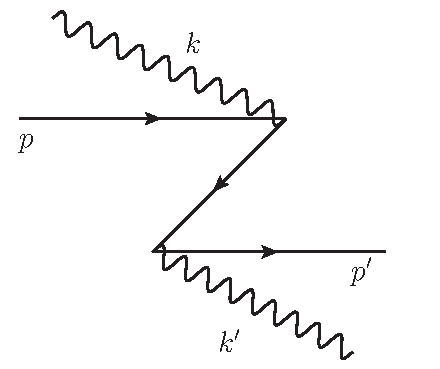
\includegraphics[scale=0.4]{eps/Zdiag} 
\end{minipage}
 = \hspace{0.5em}
\begin{minipage}{3in}
\beq
\begin{split}
	\Sigma_{\text{spin}}
	\left( 1 - \frac{k_0}{2m} \right ) &\frac{1}{2m} 
		\left[ \phi^\dagger \left( F_1 + F_2 \frac{ -k'_0}{2m} \right ) \gv{\sigma} \cdot \gv{\epsilon}^*(k') \chi \right]
\\ &	\times	\left[ \epsilon_j(k) \chi^\dagger \left( F_1 - F_2 \frac{k_0}{2m} \right)  \gv{\sigma} \cdot  \gv{\epsilon}(k)   \phi \right ]	
\end{split}
\eeq
\end{minipage}
} 
\vspace{1em}

The sum over intermediate spin spates just becomes the identity: $\Sigma_{\text{spin}} \chi^\dagger \chi = 1$. 
\beq
	= \frac{1}{2m} \left( 1 - \frac{k_0}{2m} \right ) \phi^\dagger \left[ 
			\left( F_1 - F_2 \frac{k'_0}{2m} \right )
			\left( F_1 - F_2 \frac{k_0}{2m} \right)
			\gv{\sigma} \cdot \gv{\epsilon}^*(k')  \gv{\sigma} \cdot  \gv{\epsilon}(k)  
		\right ] \phi
\eeq
	
Since only terms up to order $1/m$ are needed, this can be simplified.  Also, in this approximation $k'_0 \approx k_0$, as the total conservation of energy implies $k'_0 - k_0 = p_0 - p'_0 \sim \v{p}^2/m^2$.  So for convenience everything will be written in terms of $k_0$.  

\beq
	= \frac{1}{2m}  \phi^\dagger \left[ 
			\left( F_1^2 - F_1 [F_1 + 2 F_2 ] \frac{k_0}{2m} \right )
			\gv{\sigma} \cdot \gv{\epsilon}^*(k')  \gv{\sigma} \cdot  \gv{\epsilon}(k)  
		\right ] \phi
\eeq


The other Z diagram, coming from the crossed diagram is:

\vspace{1em}
 \mbox{
\begin{minipage}{1in}
   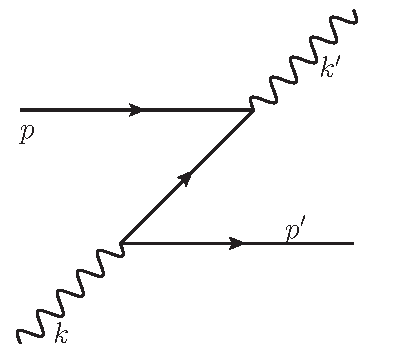
\includegraphics[scale=0.4]{eps/Zdiag2} 
\end{minipage}
= \hspace{0.5em}
$	
\Sigma_{\text{spin}}
\left( 1 + \frac{k'_0}{2m} \right ) \frac{1}{2m} 
	\left[ \phi^\dagger \left( F_1 + F_2 \frac{ k_0}{2m} \right ) \gv{\sigma} \cdot \gv{\epsilon}^(k) \chi \right]
	\left[ \epsilon_j(k) \chi^\dagger \left( F_1 + F_2 \frac{k'_0}{2m} \right)  \gv{\sigma} \cdot  \gv{\epsilon}^*(k')   \phi \right ]	
$
} 
\vspace{1em}
After summing over spin states
\beq
	= \frac{1}{2m} \left( 1 + \frac{k'_0}{2m} \right ) \phi^\dagger \left[ 
			\left( F_1 + F_2 \frac{k_0}{2m} \right )
			\left( F_1 + F_2 \frac{k'_0}{2m} \right)
			\gv{\sigma} \cdot \gv{\epsilon}^(k)  \gv{\sigma} \cdot  \gv{\epsilon}^*(k')  
		\right ] \phi
\eeq
And then applying the same simplifications as before
\beq
	= \frac{1}{2m}  \phi^\dagger \left[ 
			\left( F_1^2 + F_1 [F_1 + 2 F_2 ] \frac{k_0}{2m} \right )
			\gv{\sigma} \cdot \gv{\epsilon}^(k)  \gv{\sigma} \cdot  \gv{\epsilon}^*(k')  
		\right ] \phi
\eeq

The local interaction comes from the sum of the two diagrams.  Adding them together,

%TODO add diagram?
\mbox{
\begin{minipage}{0.6in}
   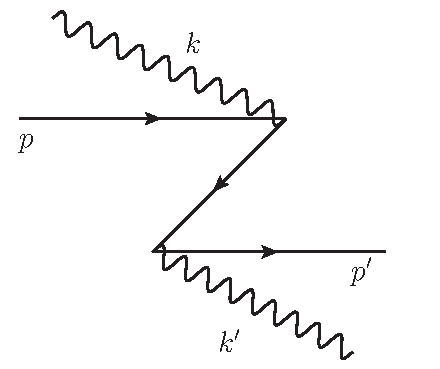
\includegraphics[scale=0.2]{eps/Zdiag} 
\end{minipage}
+
\begin{minipage}{0.6in}
   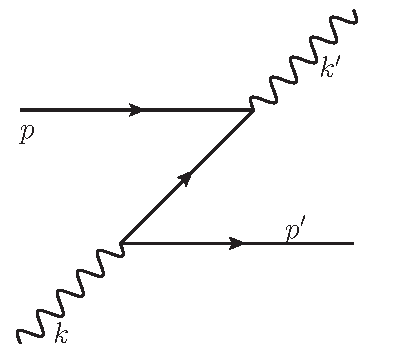
\includegraphics[scale=0.2]{eps/Zdiag2} 
\end{minipage}
\begin{minipage}{2in}
\begin{equation*}
=
\begin{split}
 & \frac{1}{2m} \phi^\dagger \Bigg [
	 \left( F_1^2 + F_1 [F_1 + 2 F_2 ] \frac{k_0}{2m} \right )
			\gv{\sigma} \cdot \gv{\epsilon}^(k)  \gv{\sigma} \cdot  \gv{\epsilon}^*(k')  \\
	&+ 
			\left( F_1^2 - F_1 [F_1 + 2 F_2 ] \frac{k_0}{2m} \right )
			\gv{\sigma} \cdot \gv{\epsilon}^*(k')  \gv{\sigma} \cdot  \gv{\epsilon}(k)  
		 \Bigg ] \phi	
\end{split}
\end{equation*}
\end{minipage}
}
\beq
\begin{split}
=&
		\frac{F_1}{2m}  \phi^\dagger \Bigg [
			F_1 \{ \gv{\sigma} \cdot \gv{\epsilon},   \gv{\sigma} \cdot  \gv{\epsilon}^* \}
			+ (F_1 + 2F_2) \frac{k_0}{2m} [ \gv{\sigma} \cdot \gv{\epsilon},   \gv{\sigma} \cdot  \gv{\epsilon}^* ]
		 \Bigg ] \phi	\\
	=&
		\frac{F_1}{m}  \phi^\dagger \Bigg [
			F_1  \gv{\epsilon} \cdot  \gv{\epsilon}^* 
			+ (F_1 + 2F_2) \frac{k_0}{2m} \gv{\sigma} \cdot \gv{\epsilon} \times  \gv{\epsilon}^* 
		 \Bigg ] \phi
\end{split}
\eeq
It now remains to calculate the same amplitude in NRQED and compare.
		
\subsection{Compton scattering in NRQED}
The idea is to calculate the Compton scattering in the nonrelativistic theory.  The gauge is chosen such that the photon polarisations obey $\epsilon_0 = 0$.  In general, both terms arising from two-photon vertices, and those from tree level diagrams of two one-photon vertices, should be considered.  However, because of the approach taken in calculating the process from the relativistic Lagrangian, only the former terms are needed.  That is, contact terms (which arise from some combination of Z-diagrams in the relativistic theory)  are separated from the rest.  

Further, ultimately only a few of these terms are relevant -- terms which have both $\v{B}$ and $\v{A}$ can be ignored.

The remaining terms of interest are:
\scriptsize
\beqa
	\mathcal{L}_{A^2} &=& \Psi^\dagger ( - \frac{e^2 \v{A}^2}{2m}  - e^2 \frac{ \{ \grad^2, \v{A}^2 \} 
}{8m^3} - e^2\frac{ \{\nabla_i, A_i \} \{\nabla_j, A_j\} }{8m^3}
		+ c^2_S \frac{ e^2 \v{S} \smalldot ( \v{A} \times \v{E} - \v{E} \times \v{A} )}{8m^2} ) \Psi
\eeqa
\normalsize

The process considered has an incoming photon with momentum $k$ and polarisation $\epsilon(k)$, and an outgoing photon with momentum $k'$ and polarisation $\epsilon^*(k')$.  The charged particle has incoming momentum $p$ and outgoing $p'= p + k - k'$.

As in the single-photon calculation, it is simply a matter of reading terms off the Lagrangian.  To find the scattering amplitude,  replace $\Psi$ with $\phis$, and replace $\v{A}$ with photon polarisations $\epsilon$ and $\epsilon^*$.  In the gauge chosen, $\v{E}(k) = -\partial_0 \v{\A} = i k_0 \gv{\epsilon}(k) = -ik'_0 \gv{\epsilon^*}(k') $ .

Contracted with the photon of momentum $k$, the result is $\v{E} \to i k_0 \v{\A}$, while with the photon of momentum $k'$ it is $\v{E} \to i k'_0 \v{\Adag}$.  Both processes must be considered in calculating the scattering, so:
\[
	\v{A} \times \v{E} = - \v{A} \times (\partial_0 \v{A})
		\to 
	-i(k_0' \v{\epsilon} \times \v{\epsilon} - k_0 \v{\epsilon} \times \v{\epsilon} ) = i ( k_0' + k_0) \v{\epsilon} \times \v{\epsilon}^*
\]
And
\[
	\v{E} \times \v{A} = - (\partial_0 \v{A}) \times  \v{A}
		\to 
	-i( k_0 \v{\epsilon} \times \v{\epsilon^*} - k_0' \v{\epsilon^*} \times \v{\epsilon} ) = -i ( k_0' + k_0) \v{\epsilon} \times \v{\epsilon^*}
\]
So from the term in the Lagrangian 
\[
 c_S \Psi^\dagger \frac{ e^2 \v{S} \smalldot ( \v{A} \times \v{E} - \v{E} \times \v{A} )}{8m^2} ) \Psi
\]
appears in the scattering amplitude
\[
  -i c_S \phi^\dagger  \Big ( \frac{e^2}{4m^2}    i(k_0 + k_0')    \v{\epsilon} \times \v{\epsilon^*} \Big ) \phi
	=
     c_S \frac{e^2}{4m^2} \phi^\dagger  \Big ( (k_0 + k_0')    \v{\epsilon} \times \v{\epsilon^*} \Big ) \phi
\]
Using the approximation $k_0 \approx k'_0$, that part of the amplitude now becomes
\beq \label{eq:Sh:ComptNR}
     c_S \frac{e^2}{2m^2} \phi^\dagger  \Big ( k_0    \v{\epsilon} \times \v{\epsilon^*} \Big ) \phi
\eeq


This is the part of the amplitude wanted to compare for reasons of consistency.
	

\subsection{Comparison of QED and NRQED Compton scattering}
Now that the amplitude has been calculated in both theories, the coefficient of NRQED $c_S$ can be fixed.  Using that $F_1 = e$ and $F_2 = e\frac{g-2}{2}$, $F_1 + 2F_2 = e^2(g-1)$.
So the final result is that 
\beq
	c_S = g-1
\eeq
 


